\documentclass[10pt]{article}
\usepackage[a4paper]{geometry}
\usepackage{amsmath}
\usepackage{amssymb}
\usepackage{tocbibind}
\usepackage{graphicx}
\usepackage{hyperref}
\usepackage{mdframed}
\usepackage{subfiles}
\usepackage{titlesec}
\usepackage[dvipsnames]{xcolor}

%%%%%%%%%%%%%%%%%%%%%%%%%%%%%%%%%%%%%%%%%%%%%%%%%%%%%%%%%%%%%%%%%%%%%%%% Setups
\newcommand{\Eq}[1]{Equation~\ref{eq:#1}}
\newcommand{\Fig}[1]{Figure~\ref{fig:#1}}

\newenvironment{textbox}[1]
{%
  \mdfsetup{%
    frametitle={\colorbox{white}{\space#1\space}},
    frametitleaboveskip=-\ht\strutbox,
  }
  \begin{mdframed}
}
{
  \end{mdframed}
}

\setlength\parindent{0pt}
\setlength\parskip{1.2ex}

\graphicspath{{./fig/}}

\hypersetup{%
  hidelinks,
  colorlinks,
  citecolor={YellowOrange!85!black},
  linkcolor={Aquamarine!85!black},
  bookmarksopen=true,
  bookmarksnumbered=true,
  linktoc=all,
  pdfauthor=Jihang Li,
}

\title{Notes of ``Object-Proposal Evaluation Protocol is `Gameable'\,''}
\author{Jihang Li}
%%%%%%%%%%%%%%%%%%%%%%%%%%%%%%%%%%%%%%%%%%%%%%%%%%%%%%%%%%%%%%%%%%%%%%%%%%%%%%%

\begin{document}
\maketitle
\tableofcontents

%%%%%%%%%%%%%%%%%%%%%%%%%%%%%%%%%%%%%%%%%%%%%%%%%%%%%%%%%%%%%%%%%%%%%% Abstract
\section*{Abstract}%
\label{sec:abstract}
The choice of using a partially annotated dataset for evaluation of object
proposals is problematic. To alleviate this problem:
%
\begin{enumerate}
  \item Introduce a nearly-fully annotated version of PASCAL VOC dataset, which
    serves as test-bed to check if object proposal techniques are over-fitting
    to a particular list of categories.
  \item Perform an exhaustive evaluation of object proposal methods on the
    introduced nearly-fully annotated PASCAL dataset and perform cross-dataset
    generalization experiments.
  \item Introduce a diagnostic experiment to detect the \textbf{bias capacity}
    in an object proposal algorithm.
\end{enumerate}

%%%%%%%%%%%%%%%%%%%%%%%%%%%%%%%%%%%%%%%%%%%%%%%%%%%%%%%%%%%%%%%%%%%%% Chapter 1
\section{Introduction}%
\label{sec:introduction}
Despite the different goals between object proposal and detection, there exists
only a single evaluation protocol:
%
\begin{enumerate}
  \item Generate proposals on a dataset.
  \item Measure the performance of the generated proposals, typically using
    recall.
\end{enumerate}

Contributions:
%
\begin{itemize}
  \item Report the ``gameability'' of the current object proposal evaluation
    protocol.
  \item Present a simple technique for producing state-of-art object proposals.
  \item Propose three ways of improving the current evaluation protocol to
    measure the category independence of object proposals:
    \begin{enumerate}
      \item Evaluation on fully annotated datasets.
      \item Cross-dataset evaluation on densely annotated datasets.
      \item A \textbf{new evaluation} metric that quantifies the
        \textbf{bias capacity} of proposal generators.
    \end{enumerate}
  \item Thoroughly evaluate existing proposal methods on this near-fully and
    two densely annotated datasets.
\end{itemize}
%
\begin{figure}[htpb]
  \centering
  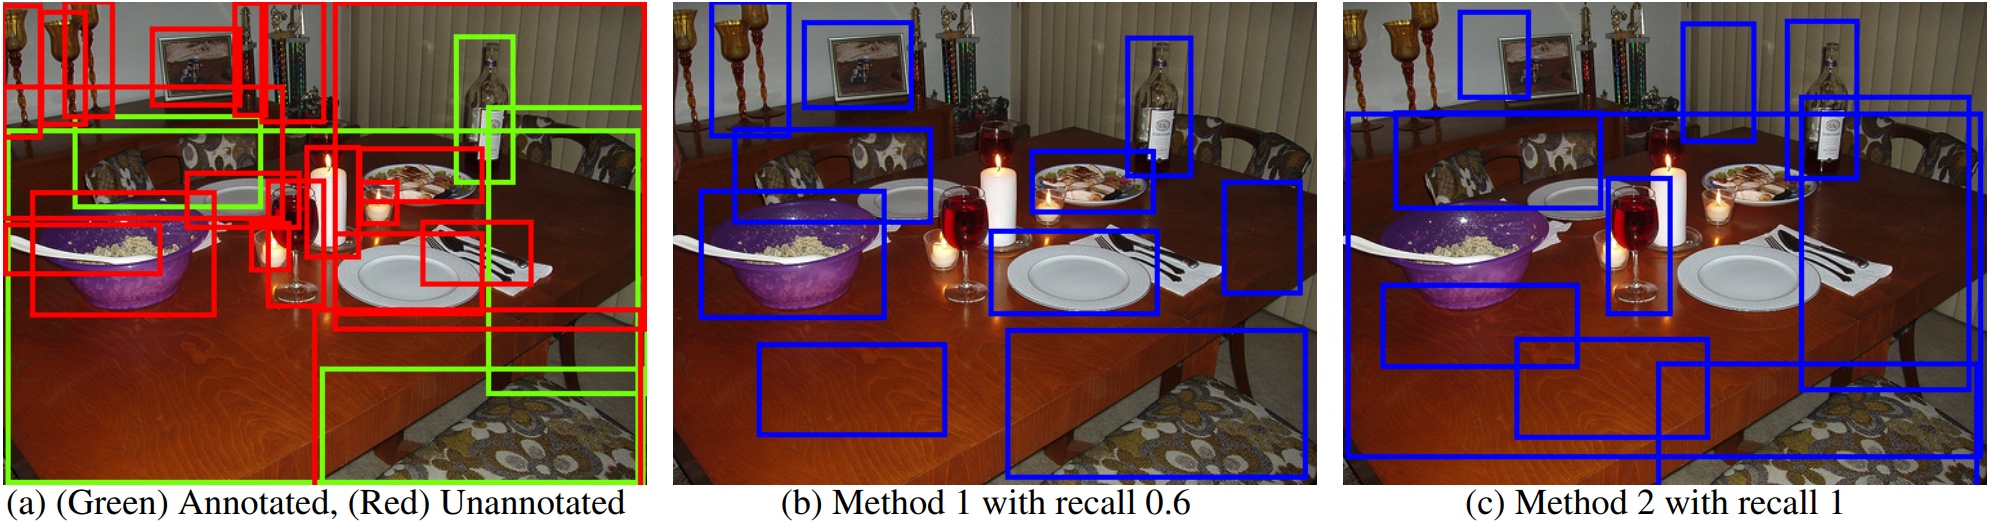
\includegraphics[width=0.8\linewidth]{fig_1.png}
  \caption{(a) shows PASCAL annotations natively present in the dataset in
    green. Other objects that are not annotated but present in the image are
    shown in red; (b) shows Method 1 and (c) shows Method 2. Method 1 visually
    seems to recall more categories such as plates, glasses, etc\. that Method
    2 missed. Despite that, the computed recall for Method 2 is higher because
    it recalled all instances of PASCAL categories that were present in the
    ground truth. Note that the number of proposals generated by both methods
    is equal in this figure.}%
  \label{fig:1}
\end{figure}

\begin{figure}[htpb]
  \centering
  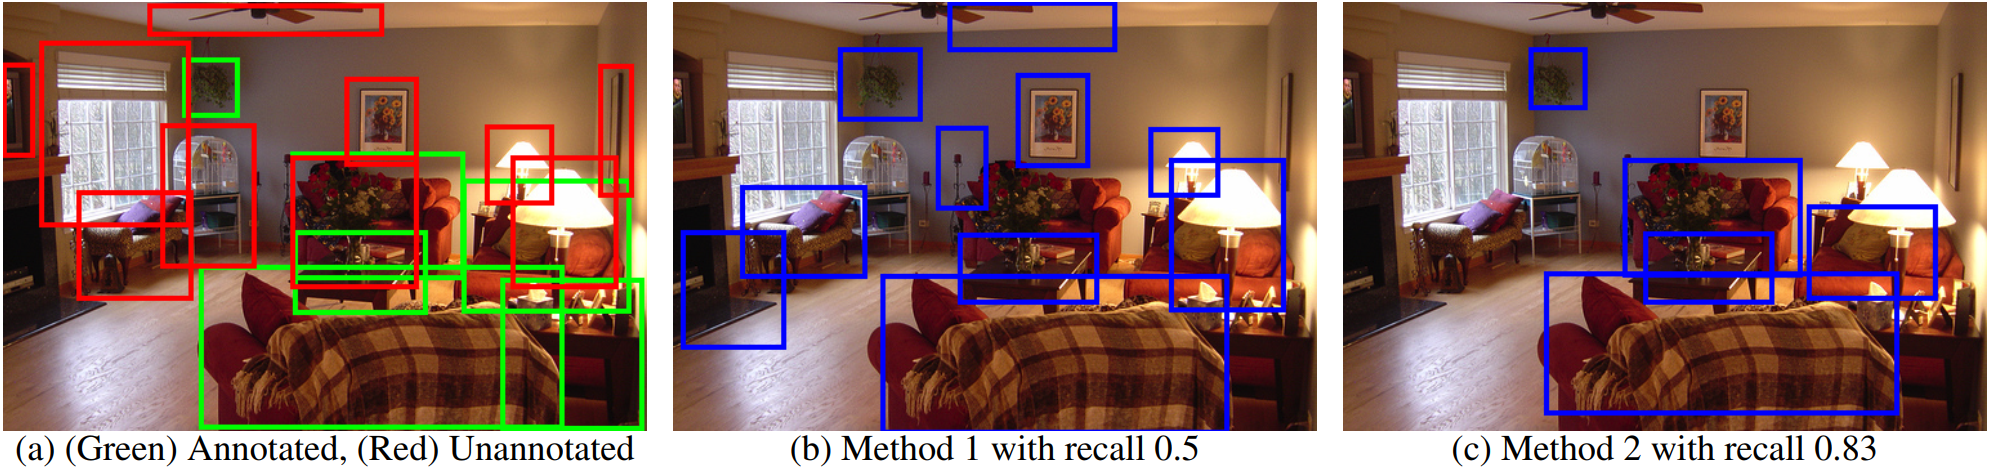
\includegraphics[width=0.8\linewidth]{fig_2.png}
  \caption{Figure 2: (a) shows PASCAL annotations natively present in the
    dataset in green. Other objects that are not annotated but present in the
    image are shown in red; (b) shows Method 1 and (c) shows Method 2. Method 1
    visually seems to recall more categories such as lamps, picture, etc.\ that
    Method 2 missed. Clearly the recall for Method 1 should be higher. However,
    the calculated}%
  \label{fig:2}
\end{figure}

%%%%%%%%%%%%%%%%%%%%%%%%%%%%%%%%%%%%%%%%%%%%%%%%%%%%%%%%%%%%%%%%%%%%% Chapter 2
\section{Related Work}%
\label{sec:related}
\textbf{Evaluating Proposals:}
%
\begin{itemize}
  \item \href{https://arxiv.org/pdf/1406.6962.pdf}{Hosang \textit{et al.}}
    focus on evaluation of object proposal algorithms, in particular the
    stability of such algorithms on parameter changes and image perturbations.
  \item \href{https://arxiv.org/pdf/1502.05082.pdf}{Hosang \textit{et al.}}
    presents an analysis of various proposal methods regarding proposal
    repeatability, ground truth annotation recall, and their impact on
    detection performance. They also introduced a new evaluation metric:
    \textbf{Average Recall}.
  \item \href{http://www.vision.ee.ethz.ch/~biwiproposals/boosting-coco/}{Pont-Tuset \textit{et al.}}
    analyzes the state-of-the-art methods in segment-based object proposals,
    focusing on the challenges faced when going from PASCAL VOC to MS COCO\@.
    Also analyzes how aligned the proposal methods are with the \textbf{bias}
    observed in MS COCO towards small objects and the center of the image and
    propose a method to boost their performance.
\end{itemize}

%%%%%%%%%%%%%%%%%%%%%%%%%%%%%%%%%%%%%%%%%%%%%%%%%%%%%%%%%%%%%%%%%%%%% Chapter 3
\section{Evaluating Object Proposals}%
\label{sec:protocols}
Widely used evaluation metrics:
%
\begin{itemize}
  \item \textbf{Recall} @ \textbf{IOU Threshold} $t$: For each ground-truth
    instance, this metric checks whether the ``best'' proposal from list $
    has IOU greater than a threshold $. If so, this ground truth instance is
    considered ``detected'' or ``recalled''. Then average recall is measured
    over all the ground truth instance:
    %
    \begin{align}
      \setcounter{equation}{1}
      \label{eq:2}
      \text{Recall @} t = \frac{1}{\vert G \vert} \sum_{g_i \in G} I[\max_{l_j \in L} \text{IOU}(g_i, l_j) > t], 
    \end{align}
    %
    where $I[\cdot]$ is an indicator function for the logical preposition in
    the argument. Object proposals are evaluated using this metric in two ways:
    %
    \begin{itemize}
      \item plotting Recall-\textit{vs.}-\#proposals by fixing $t$
      \item plotting Recall-\textit{vs.}-t by fixing the \#proposals in $L$
    \end{itemize}
  \item \textbf{Area Under the recall Curve (AUC)}: AUC summarized the area
    under the Recall-\textit{vs.}-\#proposals plot for different values of $t$
    in a single plot. This metric measures:
    %
    \begin{itemize}
      \item AUC-\textit{vs.}-\#proposals
      \item AUC-\textit{vs.}-$t$ by varying \#proposals in $L$
    \end{itemize}
  \item \textbf{Volume Under Surface (VUS)}: Measures the average recall by
    linearly varying $t$ and varying the \#proposal in $L$ on either linear or
    log scale. Thus it merges both kinds of AUC plots into one.
  \item \textbf{Average Best Overlap (ABO)}: This metric eliminates the needs
    for a threshold. The overlap between each ground truth annotation
    $g_i \in G$ and the `best' object hypotheses in $L$:
    %
    \begin{align}
      \label{eq:3}
      \text{ABO} = \frac{1}{\vert G \vert} \sum_{g_i \in G} \max_{l_j \in L} \text{IOU}(g_i, l_j)
    \end{align}
    %
    ABO is typically is calculated on a per class basis. Mean Average Best
    Overlap (MABO) is defined as the mean ABO over all classes.
  \item \textbf{Average Recall (AR)}: AR-\textit{vs.}-\#proposals (for IOU
    between 0.5 to 1) in $L$ is plotted. AR also summarizes proposal
    performance across different values of $t$. AR was shown to correlate with
    ultimate detection performance better than other metrics.
\end{itemize}

%%%%%%%%%%%%%%%%%%%%%%%%%%%%%%%%%%%%%%%%%%%%%%%%%%%%%%%%%%%%%%%%%%%%% Chapter 4
\section{A Thought Experiment: How to Game the Evaluation Protocol}%
\label{sec:experiment}
%
\begin{figure}[htpb]
  \centering
  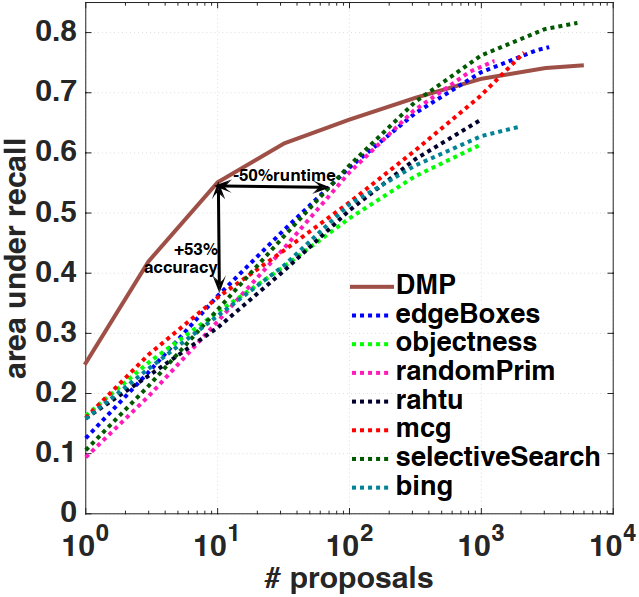
\includegraphics[width=0.8\linewidth]{fig_3.png}
  \caption{Performance of different object proposal methods (dashed lines) and
    our proposed `fraudulent' method (DMP) on the PASCAL VOC 2010 dataset. We
    can see that DMP significantly outperforms all other proposal generators.}%
  \label{fig:3}
\end{figure}

\end{document}
